\chapter{Derivatives}

% expansion:intuition — chapter overview tying the limit machinery of Ch 1 to the operator built in this chapter
The limit machinery of Chapter 1 was developed in part to make precise the idea of a function approaching a value as its input approaches some target. The principal payoff of that machinery, and the subject of this chapter, is the \emph{derivative}: an operator that takes a function and returns another function describing how fast it is changing. Geometrically the derivative gives the slope of the tangent line at each point of a curve; physically it gives the instantaneous rate of change of a quantity that varies in time; algebraically it satisfies a small set of arithmetic rules that turn differentiation into a procedure rather than a per-problem invention. We meet the derivative first at a single point as a limit of secant slopes, then as a function in its own right, then as something whose existence at a point implies (but is not implied by) continuity, and finally as an operator we can compute on polynomials, on the natural exponential, and on products and quotients of differentiable functions.

% expansion:summary — learning outcomes distilled from the manuscript's coverage. Verb-first per CONTENT_QUICKSTART.
\paragraph{By the end of this chapter, you will be able to:}
\begin{itemize}
    \item state the limit definition of the derivative and apply it to compute derivatives from first principles for polynomial, root, and exponential functions;
    \item move fluently between the equivalent forms \(\lim_{x \to a} \tfrac{f(x) - f(a)}{x - a}\) and \(\lim_{h \to 0} \tfrac{f(a + h) - f(a)}{h}\);
    \item recognise where a function fails to be differentiable, and explain why differentiability implies continuity but not the reverse;
    \item compute higher-order derivatives \(f''\), \(f'''\), and \(f^{(n)}\);
    \item differentiate any polynomial and the exponential function \(e^{x}\) using the power rule, the constant-multiple rule, the sum rule, and the series-based derivation of \((e^{x})' = e^{x}\);
    \item differentiate products and quotients of differentiable functions using the product and quotient rules.
\end{itemize}

\section{The Tangent Line and the Derivative at a Point}\label{sec:derivative-at-a-point}

% expansion:intuition — section opener motivating the tangent line as the geometric object whose slope we want to capture, and previewing the secant-to-tangent limit
A common geometric question about a curve \(y = f(x)\) is: at a chosen point \(P = (a, f(a))\) on the curve, what is the equation of the line that just touches the curve at \(P\) without crossing through it locally? This is the tangent line at \(P\), and it has many uses. Far from being a purely geometric curiosity, the tangent line is the linear approximation of the curve near \(P\): close enough to \(P\), the curve and its tangent line are visually indistinguishable, and computations about the curve can be replaced by computations about a line. To find the tangent line, we need its slope, since the line already passes through the known point \(P\). Finding the slope is the work of this section, and the answer turns out to be a limit.

\subsection{Secant slopes and their limit}

Take a second point on the curve, \(Q = (x, f(x))\) with \(x\) near \(a\) but not equal to \(a\). The line through \(P\) and \(Q\) is a \emph{secant line}\index{secant line}; its slope is the difference quotient
\[
m_{PQ} = \frac{f(x) - f(a)}{x - a}.
\]
As \(Q\) slides along the curve toward \(P\), the secant line pivots toward what we want to call the tangent line, and its slope pivots toward the tangent slope. \Cref{fig:secant-to-tangent} shows three secant lines for successively closer values of \(x\); their pivot point is \(P\), and their limiting position --- the tangent at \(P\) --- is drawn in red.

\begin{figure}[H]
\centering
\begin{tikzpicture}[scale=1.05]
\draw[->] (-0.3,0) -- (4.6,0) node[right] {$x$};
\draw[->] (0,-0.3) -- (0,3.4) node[above] {$y$};
% The curve y = 0.4x^2 + 0.6 from x=0.5 to x=4.2
\draw[blue, thick, domain=0.4:4.2, samples=80] plot (\x,{0.4*\x*\x*0.5 + 0.7});
\node[blue, right] at (4.2,{0.4*4.2*4.2*0.5 + 0.7}) {$y = f(x)$};
% Point P = (1.5, f(1.5))
\fill (1.5,{0.4*1.5*1.5*0.5 + 0.7}) circle (1.8pt);
\node[below] at (1.5,{0.4*1.5*1.5*0.5 + 0.45}) {$P = (a, f(a))$};
% Three secants from P to (3.6, .), (2.8, .), (2.2, .)
\foreach \x in {3.6, 2.8, 2.2} {
  \draw[gray, thin]
    ($(1.5,{0.4*1.5*1.5*0.5 + 0.7})!-0.4!(\x,{0.4*\x*\x*0.5 + 0.7})$)
    --
    ($(1.5,{0.4*1.5*1.5*0.5 + 0.7})!1.3!(\x,{0.4*\x*\x*0.5 + 0.7})$);
  \fill[gray] (\x,{0.4*\x*\x*0.5 + 0.7}) circle (1.3pt);
}
\node[gray, right] at (3.65,{0.4*3.6*3.6*0.5 + 0.7}) {$Q$};
% Tangent at P: slope = 0.4 * 1.5 = 0.6
\draw[red, thick]
  ($(1.5,{0.4*1.5*1.5*0.5 + 0.7})!-1.3!(1.5+1,{0.4*1.5*1.5*0.5 + 0.7 + 0.6})$)
  --
  ($(1.5,{0.4*1.5*1.5*0.5 + 0.7})!1.6!(1.5+1,{0.4*1.5*1.5*0.5 + 0.7 + 0.6})$);
\node[red, right] at (3.0,{0.4*1.5*1.5*0.5 + 0.7 + 0.6 + 0.7}) {tangent at $P$};
\end{tikzpicture}
\caption{Secant lines through \(P\) and a second point \(Q\) pivot toward the tangent at \(P\) as \(Q\) approaches \(P\) along the curve.}
\label{fig:secant-to-tangent}
\end{figure}

This pivoting is exactly the kind of limit we developed in Chapter 1: as \(x \to a\), the secant slope \(m_{PQ}\) approaches the tangent slope at \(P\), provided this limit exists. We adopt this as the definition of the tangent line.

\begin{definition}\label{def:tangent-line}
The \emph{tangent line}\index{tangent line} to the curve \(y = f(x)\) at the point \(P = (a, f(a))\) is the line through \(P\) with slope
\[
m = \lim_{x \to a} \frac{f(x) - f(a)}{x - a},
\]
provided this limit exists. When the limit fails to exist, we say the curve has no tangent line at \(P\).

% expansion:intuition — Informally gloss
\emph{Informally, the tangent line at \(P\) is the limiting position of secant lines through \(P\) as the second point slides toward \(P\).}
\end{definition}

% expansion:caution — the popular "touches the curve at one point" picture is geometrically wrong; flagging this once now saves rework later
\begin{caution}
A common informal description of the tangent line --- ``the line that touches the curve at exactly one point'' --- is not the right idea. A line can touch a curve at one point without being tangent to it (a vertical line touches \(y = x^{3}\) at one point but is not its tangent), and a tangent line can touch the curve at more than one point: the horizontal tangent to \(y = x^{3} - 3x\) at the local maximum \(x = -1\) is the line \(y = 2\), and that line meets the curve again at \(x = 2\) (since \(x^{3} - 3x - 2 = (x + 1)^{2}(x - 2)\)). The mathematically correct picture is the limiting-secant one of \cref{def:tangent-line}: we ask for the line whose slope is the limit of nearby secant slopes, not for the line that ``touches at one point''.
\end{caution}

% expansion:figure — the manuscript's "zoom in" remark deserves its own diagram. Standard textbook content; emphasises that the tangent line is the local linearisation.
\begin{figure}[H]
\centering
\begin{tikzpicture}[scale=0.9]
% Three panels showing increasing zoom on the same curve at the same point
\foreach \k/\zoom in {0/1, 1/2.5, 2/6} {
\begin{scope}[xshift=\k*4cm]
\draw[->] (-1.5/\zoom,0) -- (1.5/\zoom,0);
\draw[->] (0,-1.5/\zoom) -- (0,1.5/\zoom);
\draw[blue, thick, domain=-1.4/\zoom:1.4/\zoom, samples=80] plot (\x,{0.6*\x*\x});
\draw[red, thick, domain=-1.4/\zoom:1.4/\zoom, samples=2] plot (\x,{0});
\fill (0,0) circle (1.5pt);
\node[below] at (0,-1.5/\zoom-0.05) {$\zoom\times$};
\end{scope}
}
\end{tikzpicture}
\caption{Zooming in at \(P\): the curve and its tangent line become visually indistinguishable. This is what makes the tangent line a useful local linear approximation of the curve.}
\label{fig:tangent-zoom}
\end{figure}

\subsection{The equivalent \texorpdfstring{$h$}{h}-form}

Setting \(x = a + h\) makes \(x \to a\) equivalent to \(h \to 0\), and substituting transforms the difference quotient:
\[
\frac{f(x) - f(a)}{x - a} = \frac{f(a + h) - f(a)}{h}.
\]
The \emph{\(h\)-form} below is therefore equivalent to the form in \cref{def:tangent-line}, and is the form most often used in computation.

\begin{proposition}\label{prop:tangent-h-form}
The slope of the tangent line at \((a, f(a))\) is also given by
\[
m = \lim_{h \to 0} \frac{f(a + h) - f(a)}{h},
\]
whenever this limit exists.
\end{proposition}

% expansion:caution — equivalence of the two forms is conceptually clean but a substitution students often perform mechanically. Worth flagging that h can be positive or negative.
\begin{caution}
In the \(h\)-form, \(h\) ranges over both positive and negative values --- a positive \(h\) places \(Q\) to the right of \(P\), a negative \(h\) places it to the left, and the limit \(h \to 0\) requires both sides to give the same value. The condition ``\(x\) near \(a\) but \(x \neq a\)'' from \cref{def:tangent-line} translates exactly to ``\(h\) near \(0\) but \(h \neq 0\)''.
\end{caution}

\subsection{Computing a tangent line}

The two forms above turn the geometric question (find the tangent line) into a procedural one (compute a limit, then write the line equation). The next strategy distils the steps; the worked examples illustrate the strategy on increasingly nontrivial functions.

% expansion:strategy — the section's core procedure made into a project strategy box
\begin{strategy}[Finding the tangent line at \((a, f(a))\)]
To find the tangent line to \(y = f(x)\) at \(x = a\):
\begin{enumerate}
    \item Compute the slope by evaluating one of the two equivalent limits
    \[
    m = \lim_{x \to a} \frac{f(x) - f(a)}{x - a}
    \qquad \text{or} \qquad
    m = \lim_{h \to 0} \frac{f(a + h) - f(a)}{h}.
    \]
    The \(h\)-form is usually easier when \(f\) is given by a polynomial or a simple algebraic expression; the \(x\)-form is usually easier when \(f\) involves a quotient or root that is easier to subtract directly.
    \item Use the point-slope form \(y - f(a) = m \cdot (x - a)\) to write the line equation.
    \item Simplify to slope-intercept or general form as the problem requires.
\end{enumerate}
If the limit in step 1 fails to exist, the curve has no tangent line at the point. The standard culprits are corners (one-sided limits exist but disagree, e.g.\ \(y = \lvert x \rvert\) at \(x = 0\)) and vertical tangents (the limit is \(\pm \infty\), e.g.\ \(y = \sqrt[3]{x}\) at \(x = 0\)).
\end{strategy}

\begin{workedexample}
\begin{example}\label{ex:tangent-3-over-x}
Find the tangent line to the curve \(y = \dfrac{3}{x}\) (with \(x > 0\)) at the point \((3, 1)\).
\end{example}

\begin{solution}
With \(f(x) = 3/x\) and \(a = 3\), the \(h\)-form gives
\begin{aligneddisplay}
m &= \lim_{h \to 0} \frac{f(3 + h) - f(3)}{h}
   = \lim_{h \to 0} \frac{1}{h}\left(\frac{3}{3 + h} - 1\right) \\
  &= \lim_{h \to 0} \frac{1}{h} \cdot \frac{3 - (3 + h)}{3 + h}
   = \lim_{h \to 0} \frac{1}{h} \cdot \frac{-h}{3 + h} \\
  &= \lim_{h \to 0} \frac{-1}{3 + h} = -\frac{1}{3}.
\end{aligneddisplay}
The tangent at \((3, 1)\) is therefore the line \(y - 1 = -\tfrac{1}{3}(x - 3)\), which simplifies to
\[
x + 3y - 6 = 0. \qedhere
\]
\end{solution}
\end{workedexample}

% expansion:example — supplementary linear example. Verifies that the construction returns the expected slope when the curve already is a line.
\begin{workedexample}
\begin{example}
Find the tangent line to \(y = 4x - 5\) at any point \((a, 4a - 5)\).
\end{example}

\begin{solution}
With \(f(x) = 4x - 5\),
\[
m = \lim_{h \to 0} \frac{f(a + h) - f(a)}{h}
  = \lim_{h \to 0} \frac{4(a + h) - 5 - (4a - 5)}{h}
  = \lim_{h \to 0} \frac{4h}{h}
  = 4.
\]
The tangent line at any point on the line \(y = 4x - 5\) has slope \(4\) and passes through the chosen point; it is therefore the line itself. The construction is consistent with what we already know: a straight line is its own tangent at every point.
\end{solution}
\end{workedexample}

% expansion:example — the canonical parabola tangent. Pedagogically central; gives a simple polynomial slope formula and prepares the §2.2 calculation of f' as a function.
\begin{workedexample}
\begin{example}\label{ex:tangent-parabola}
Find the tangent line to \(y = x^{2}\) at \((1, 1)\), and at the origin \((0, 0)\).
\end{example}

\begin{solution}
At \((a, a^{2})\) with \(a\) general,
\begin{aligneddisplay}
m &= \lim_{h \to 0} \frac{(a + h)^{2} - a^{2}}{h}
   = \lim_{h \to 0} \frac{a^{2} + 2ah + h^{2} - a^{2}}{h} \\
  &= \lim_{h \to 0} (2a + h) = 2a.
\end{aligneddisplay}
At \(a = 1\) the slope is \(2\), so the tangent is \(y - 1 = 2(x - 1)\), i.e.\ \(y = 2x - 1\). At \(a = 0\) the slope is \(0\), so the tangent is the horizontal line \(y = 0\) --- the parabola's vertex tangent.
\end{solution}
\end{workedexample}

% expansion:application [pass: enrichment] — gives the physical reading of the secant-to-tangent limit; the chapter overview promises an instantaneous-rate-of-change interpretation but \S2.1 itself develops only the tangent-slope geometry
\paragraph{Velocity as an instantaneous rate of change.}
The same limit that produced the tangent-line slope captures a familiar physical idea: instantaneous velocity. If \(s(t)\) describes the position of a moving object at time \(t\), the average velocity over the time interval \([t_{0},\, t_{0} + h]\) is the displacement divided by the elapsed time,
\[
\overline{v}_{[t_{0},\, t_{0} + h]} = \frac{s(t_{0} + h) - s(t_{0})}{h}.
\]
This is the difference quotient of \cref{prop:tangent-h-form} in physical clothing. The instantaneous velocity at \(t_{0}\) is the limit as the elapsed time shrinks,
\[
v(t_{0}) = \lim_{h \to 0} \frac{s(t_{0} + h) - s(t_{0})}{h}.
\]
Geometrically this is the slope of the tangent line to the position-versus-time graph at \(t = t_{0}\); physically it is the speedometer reading at the instant \(t_{0}\). The two views are the same calculation. For instance, an object falling from rest under gravity has position \(s(t) = \tfrac{1}{2} g t^{2}\); the parabola limit of \cref{ex:tangent-parabola} (with \(a\) renamed to \(t_{0}\) and a constant factor \(\tfrac{1}{2} g\) carried through) gives \(v(t_{0}) = g t_{0}\), the familiar formula that the velocity of a freely falling object grows linearly with time.

% expansion:summary — pulls the parabola example forward: the slope formula 2a is itself a function of a. This is exactly the bridge to §2.2.
The parabola calculation in \cref{ex:tangent-parabola} produced more than a single tangent line: it produced a \emph{formula}, \(m = 2a\), giving the slope at any point of the curve. The right-hand side is itself a function of \(a\), and storing slopes as a function rather than computing them point-by-point is the conceptual move that turns the tangent-line construction into something one differentiates rather than something one re-evaluates. The next section makes this move official.

\section{The Derivative as a Function}\label{sec:derivative-as-function}

% expansion:intuition — section opener pivoting from §2.1's "slope formula 2a is a function of a" observation
\Cref{ex:tangent-parabola} computed the tangent slope at every point of the parabola in a single calculation, producing the formula \(m = 2a\). The slope is now a function of the basepoint, and we can ask its value at any \(a\) we like without redoing the limit. Generalising this move --- treating the basepoint as a variable and recording the resulting slope formula as a function in its own right --- is the subject of this section. The function we obtain is called the derivative of \(f\), and it is the central object of the chapter.

\subsection{The derivative at a point}

We first name the limit that the previous section computed.

\begin{definition}\label{def:derivative-at-a}
The \emph{derivative}\index{derivative!at a point} of \(f\) at the point \(a\), denoted \(f'(a)\), is
\[
f'(a) = \lim_{h \to 0} \frac{f(a + h) - f(a)}{h},
\]
provided this limit exists. Equivalently, by the substitution \(x = a + h\),
\[
f'(a) = \lim_{x \to a} \frac{f(x) - f(a)}{x - a}.
\]

% expansion:intuition — Informally gloss
\emph{Informally, \(f'(a)\) is the slope of the tangent line to the graph of \(f\) at the point \((a, f(a))\), or equivalently the instantaneous rate of change of \(f\) at \(a\).}
\end{definition}

The two displayed limits in \cref{def:derivative-at-a} compute the same number whenever either exists; the choice between them is a matter of convenience for the algebra in any particular calculation.

\begin{workedexample}
\begin{example}\label{ex:derivative-quadratic}
Let \(f(x) = x^{2} + 4x - 2\). Find \(f'(a)\) for an arbitrary point \(a\).
\end{example}

\begin{solution}
The \(h\)-form of the difference quotient gives
\begin{aligneddisplay}
\frac{f(a + h) - f(a)}{h}
&= \frac{\bigl[(a + h)^{2} + 4(a + h) - 2\bigr] - \bigl[a^{2} + 4a - 2\bigr]}{h} \\
&= \frac{(a^{2} + 2ah + h^{2} + 4a + 4h - 2) - (a^{2} + 4a - 2)}{h} \\
&= \frac{2ah + h^{2} + 4h}{h}
 = 2a + h + 4.
\end{aligneddisplay}
Taking \(h \to 0\),
\[
f'(a) = \lim_{h \to 0} (2a + h + 4) = 2a + 4. \qedhere
\]
\end{solution}
\end{workedexample}

The right-hand side \(2a + 4\) is again a function of \(a\), so we can promote \(a\) to a variable and treat the entire formula as a new function.

\subsection{The derivative as a function}

\begin{definition}\label{def:derivative-function}
Let \(f\) be defined on an interval. The \emph{derivative function}\index{derivative!as a function} of \(f\), denoted \(f'\), is the function whose value at \(x\) is
\[
f'(x) = \lim_{h \to 0} \frac{f(x + h) - f(x)}{h},
\]
defined for every \(x\) at which this limit exists.

% expansion:intuition — Informally gloss
\emph{Informally, \(f'\) is the function that records the slope of \(f\) at every point where the slope is well defined.}
\end{definition}

% expansion:caution — the four common notations students will see, introduced together so the equivalence is unmistakable
\begin{caution}[Notation for the derivative]
The same object \(f'(x)\) is written in several conventional ways:
\pairdisplay{f'(x), \quad \frac{df}{dx}, \quad \frac{dy}{dx}\ (\text{when } y = f(x)),}{\frac{d}{dx}\bigl[f(x)\bigr], \quad Df.}
The notation \(\frac{dy}{dx}\) (read ``\(dy\) over \(dx\)'') is the \emph{Leibniz notation}\index{Leibniz notation}\index{notation!Leibniz}; \(f'(x)\) is the \emph{prime notation}\index{prime notation}\index{notation!prime}. The two are interchangeable. Leibniz notation is convenient when the input variable is named explicitly (e.g.\ a position function depending on time \(t\) makes \(\frac{dx}{dt}\) the natural slot for the velocity), and prime notation is convenient when the function is named without committing to a variable. The bracketed operator form \(\frac{d}{dx}[f(x)]\) is useful when the function expression is too long to give a single name, e.g.\ \(\frac{d}{dx}[x^{3} + \sin x]\). Treat \(\frac{dy}{dx}\) as a single symbol, not as a quotient of two separate quantities \(dy\) and \(dx\); the analogy with a fraction is suggestive and useful, but the symbol is defined by the limit, not by an arithmetic operation on \(dy\) and \(dx\).
\end{caution}

The procedure for computing \(f'(x)\) from the definition is the obvious adaptation of the strategy in §\ref{sec:derivative-at-a-point}: replace the fixed basepoint \(a\) by a variable \(x\) and run the limit.

% expansion:strategy — the procedure used in every worked example below; also the "first principles" technique that students will be asked to perform on standardised problems
\begin{strategy}[Computing \(f'(x)\) from the limit definition]
To compute \(f'(x)\) directly from \cref{def:derivative-function}:
\begin{enumerate}
    \item Form the difference quotient \(\dfrac{f(x + h) - f(x)}{h}\).
    \item Simplify algebraically until the factor of \(h\) in the denominator cancels --- by polynomial expansion, by rationalisation of a square root, by combining fractions over a common denominator, or by whatever algebraic device the form of \(f\) suggests.
    \item Take \(h \to 0\) on the simplified expression.
\end{enumerate}
The middle step is where the work happens; the limit at the end is usually a direct substitution once the cancellation has eliminated the denominator's \(h\). When step 2 will not produce a cancellation no matter how the algebra is rearranged, the derivative most likely does not exist (a corner, vertical tangent, or jump). \Cref{sec:differentiability-continuity} catalogues the failure modes.
\end{strategy}

\begin{workedexample}
\begin{example}\label{ex:derivative-sqrt-x}
Let \(f(x) = \sqrt{x}\) for \(x > 0\). Find \(f'(x)\).
\end{example}

\begin{solution}
The difference quotient is
\[
\frac{\sqrt{x + h} - \sqrt{x}}{h}.
\]
Multiplying numerator and denominator by the conjugate \(\sqrt{x + h} + \sqrt{x}\) rationalises the numerator:
\begin{aligneddisplay}
\frac{\sqrt{x + h} - \sqrt{x}}{h}
&= \frac{(\sqrt{x + h} - \sqrt{x})(\sqrt{x + h} + \sqrt{x})}{h(\sqrt{x + h} + \sqrt{x})} \\
&= \frac{(x + h) - x}{h(\sqrt{x + h} + \sqrt{x})}
 = \frac{1}{\sqrt{x + h} + \sqrt{x}}.
\end{aligneddisplay}
Taking \(h \to 0\),
\[
f'(x) = \lim_{h \to 0} \frac{1}{\sqrt{x + h} + \sqrt{x}}
      = \frac{1}{2\sqrt{x}}. \qedhere
\]
\end{solution}
\end{workedexample}

% expansion:example — supplementary basic-but-important example. The constant function differentiates to zero is the trivial baseline; including it before the more elaborate computations makes the "h cancels and the limit is direct substitution" pattern clear.
\begin{workedexample}
\begin{example}\label{ex:derivative-constant}
Let \(f(x) = c\) for some constant \(c\). Find \(f'(x)\).
\end{example}

\begin{solution}
The difference quotient is
\[
\frac{f(x + h) - f(x)}{h} = \frac{c - c}{h} = 0
\]
for every \(h \neq 0\). Therefore \(f'(x) = \lim_{h \to 0} 0 = 0\) for every \(x\). A constant function has zero derivative everywhere, in agreement with the geometric picture: the graph of a constant function is a horizontal line, which has slope \(0\) at every point.
\end{solution}
\end{workedexample}

% expansion:example — supplementary cubic example. Foreshadows the §2.4 power rule and gives a third independent derivation pattern (binomial expansion of the cube).
\begin{workedexample}
\begin{example}\label{ex:derivative-cubic}
Let \(f(x) = x^{3}\). Find \(f'(x)\).
\end{example}

\begin{solution}
Expand \((x + h)^{3} = x^{3} + 3x^{2} h + 3x h^{2} + h^{3}\) and substitute:
\begin{aligneddisplay}
\frac{(x + h)^{3} - x^{3}}{h}
&= \frac{3x^{2} h + 3x h^{2} + h^{3}}{h} \\
&= 3x^{2} + 3x h + h^{2}.
\end{aligneddisplay}
The factor of \(h\) has cancelled. Taking \(h \to 0\),
\[
f'(x) = \lim_{h \to 0} \bigl(3x^{2} + 3x h + h^{2}\bigr) = 3x^{2}.
\]
This together with the earlier results \((x^{2})' = 2x\) and the constant rule suggests a pattern --- \((x^{n})' = n x^{n - 1}\) --- that we will prove for every positive integer \(n\) in \cref{sec:polynomial-exponential-derivatives}.
\end{solution}
\end{workedexample}

% expansion:figure — the canonical "f and f' on aligned axes" picture, called out in the roadmap as the key §2.2 figure
\begin{figure}[H]
\centering
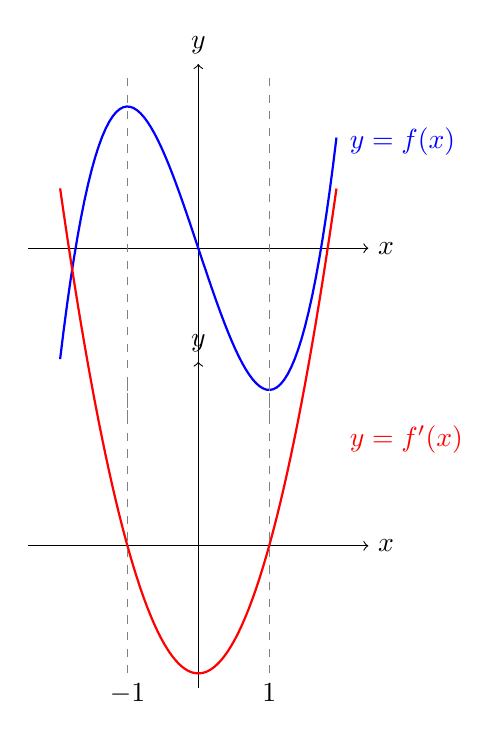
\begin{tikzpicture}[scale=0.9]
% Top panel: f(x) = x^3 - 3x
\begin{scope}[yshift=2.6cm]
\draw[->] (-2.4,0) -- (2.4,0) node[right] {$x$};
\draw[->] (0,-2.6) -- (0,2.6) node[above] {$y$};
\draw[blue, thick, domain=-1.95:1.95, samples=80] plot (\x,{\x*\x*\x - 3*\x});
\draw[gray, dashed] (-1,-2.4) -- (-1,2.4);
\draw[gray, dashed] (1,-2.4) -- (1,2.4);
\node[blue, right] at (2.0,1.5) {$y = f(x)$};
\node[below] at (-1,-2.4) {};
\node[below] at (1,-2.4) {};
\end{scope}
% Bottom panel: f'(x) = 3x^2 - 3
\begin{scope}[yshift=-1.6cm]
\draw[->] (-2.4,0) -- (2.4,0) node[right] {$x$};
\draw[->] (0,-2.0) -- (0,2.6) node[above] {$y$};
\draw[red, thick, domain=-1.95:1.95, samples=80] plot (\x,{0.6*(3*\x*\x - 3)});
\draw[gray, dashed] (-1,-1.8) -- (-1,2.4);
\draw[gray, dashed] (1,-1.8) -- (1,2.4);
\node[red, right] at (2.0,1.5) {$y = f'(x)$};
\node[below] at (-1,-1.8) {$-1$};
\node[below] at (1,-1.8) {$1$};
\end{scope}
\end{tikzpicture}
\caption{A function \(f\) (top) and its derivative \(f'\) (bottom), drawn on aligned \(x\)-axes for \(f(x) = x^{3} - 3x\), \(f'(x) = 3x^{2} - 3\). The zeros of \(f'\) (at \(x = \pm 1\)) line up with the local extrema of \(f\); the sign of \(f'\) records whether \(f\) is rising or falling.}
\label{fig:f-and-fprime-aligned}
\end{figure}

\subsection{Differentiability}

For some functions, the limit defining \(f'(x)\) fails to exist at one or more points. We give failure cases the standard name.

\begin{definition}\label{def:differentiable}
A function \(f\) is \emph{differentiable}\index{differentiable!at a point} at \(a\) if \(f'(a)\) exists. We say \(f\) is \emph{differentiable on an interval}\index{differentiable!on an interval} \((a, b)\) if it is differentiable at every point of that interval.

% expansion:intuition — Informally gloss
\emph{Informally, \(f\) is differentiable at \(a\) when its graph has a well-defined non-vertical tangent line at \((a, f(a))\); a graph that has a corner, a cusp, or a vertical tangent at the point is not differentiable there.}
\end{definition}

The next section catalogues the standard failures of differentiability and connects differentiability to continuity.

% expansion:summary — closing synthesis paragraph linking to §2.3
We have moved from a single-point construction (the tangent slope at one specific \(P\)) to a function-level construction (the derivative \(f'\) recording the slope at every basepoint where the slope is defined). The next question is when the limit defining \(f'(a)\) actually exists, and what relation that has to other regularity properties of \(f\) such as continuity. \Cref{sec:differentiability-continuity} answers both: differentiability is a strictly stronger condition than continuity.

\section{Differentiability, Continuity, and Higher Derivatives}\label{sec:differentiability-continuity}

% expansion:intuition — section opener pivoting from §2.2's preview "the limit defining f'(a) may fail to exist"
The limit defining \(f'(a)\) does not always exist. A function may be perfectly well-defined and even continuous at \(a\) yet still fail to have a derivative there, because the secant slopes from the two sides do not agree. This section catalogues the standard ways differentiability can fail, proves the basic positive result tying differentiability to continuity, and introduces the iterated derivatives \(f''\), \(f'''\), \(f^{(n)}\) that we will need in later chapters when we discuss concavity and Taylor series.

\subsection{A function that fails to be differentiable}

The cleanest example of non-differentiability is the absolute-value function at the origin.

\begin{workedexample}
\begin{example}\label{ex:abs-not-differentiable}
Show that \(f(x) = \lvert x \rvert\) is not differentiable at \(x = 0\).
\end{example}

\begin{solution}
At \(x = 0\) the difference quotient is
\[
\frac{f(0 + h) - f(0)}{h} = \frac{\lvert h \rvert - 0}{h} = \frac{\lvert h \rvert}{h}.
\]
For \(h > 0\), \(\lvert h \rvert = h\) and the quotient equals \(+1\); for \(h < 0\), \(\lvert h \rvert = -h\) and the quotient equals \(-1\). Therefore
\pairdisplay{\lim_{h \to 0^{+}} \frac{\lvert h \rvert}{h} = +1,}{\lim_{h \to 0^{-}} \frac{\lvert h \rvert}{h} = -1.}
The two one-sided limits exist but disagree, so the two-sided limit does not exist; \(f\) is not differentiable at \(0\). Geometrically, the graph has a sharp \emph{corner}\index{corner (graph)} at the origin, and there is no single tangent line that can serve both the line \(y = x\) (for \(x > 0\)) and the line \(y = -x\) (for \(x < 0\)).
\end{solution}
\end{workedexample}

\begin{figure}[H]
\centering
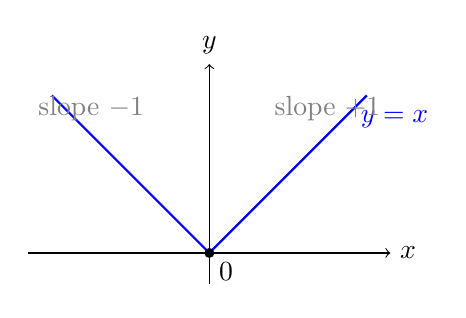
\begin{tikzpicture}[scale=1.0]
\draw[->] (-2.3,0) -- (2.3,0) node[right] {$x$};
\draw[->] (0,-0.4) -- (0,2.4) node[above] {$y$};
\draw[blue, thick] (-2,2) -- (0,0) -- (2,2);
\fill (0,0) circle (1.8pt);
\node[blue, right] at (1.8,1.7) {$y = \lvert x \rvert$};
\node[below right] at (0,0) {$0$};
% Slope labels
\node[gray, above] at (-1.5,1.55) {slope $-1$};
\node[gray, above] at (1.5,1.55) {slope $+1$};
\end{tikzpicture}
\caption{The graph of \(\lvert x \rvert\). The slopes from the left (\(-1\)) and right (\(+1\)) of the origin disagree, so \(\lvert x \rvert\) is not differentiable at \(0\).}
\label{fig:abs-corner}
\end{figure}

% expansion:strategy — non-differentiability comes in three flavours that look different on the graph; cataloguing them helps students recognise each
\begin{strategy}[Recognising non-differentiability]
A function \(f\) can fail to be differentiable at \(a\) for one of three geometric reasons:
\begin{enumerate}
    \item \emph{Corner}: the one-sided limits of the difference quotient exist but disagree (as for \(\lvert x \rvert\) at \(0\)). The graph has two distinct slopes meeting at a point.
    \item \emph{Vertical tangent}: the difference quotient diverges to \(+\infty\) or \(-\infty\) as \(h \to 0\) (e.g.\ \(f(x) = \sqrt[3]{x}\) at \(0\), where the cube-root curve has a vertical slope at the origin). The tangent line, if drawn, would be vertical, and a vertical line has no finite slope.
    \item \emph{Discontinuity}: \(f\) is not even continuous at \(a\), so the difference quotient diverges or oscillates without limit.
\end{enumerate}
The first two cases (corner and vertical tangent) involve continuous functions; the third does not. The relation between continuity and differentiability is the subject of the theorem below.
\end{strategy}

\subsection{Differentiability implies continuity}

The corner of \(\lvert x \rvert\) shows that continuity does not imply differentiability: \(\lvert x \rvert\) is continuous everywhere but not differentiable at \(0\). The reverse implication, however, does hold.

\begin{theorem}\label{thm:differentiable-implies-continuous}
If \(f\) is differentiable at \(a\), then \(f\) is continuous at \(a\).
\end{theorem}

\begin{proof}
We must show \(\lim_{x \to a} f(x) = f(a)\), or equivalently \(\lim_{x \to a} (f(x) - f(a)) = 0\). For \(x \neq a\) we can rewrite
\[
f(x) - f(a) = \frac{f(x) - f(a)}{x - a} \cdot (x - a).
\]
By assumption, the first factor approaches \(f'(a)\) as \(x \to a\); the second factor approaches \(0\). Both limits exist, so by the product law for limits,
\[
\lim_{x \to a} (f(x) - f(a)) = f'(a) \cdot 0 = 0.
\]
Hence \(\lim_{x \to a} f(x) = f(a)\), and \(f\) is continuous at \(a\).
\end{proof}

% expansion:caution — the converse is false; this is the highest-traffic misconception in the section
\begin{caution}
\Cref{thm:differentiable-implies-continuous} runs only one way: differentiable implies continuous, but \emph{continuous does not imply differentiable}. The function \(\lvert x \rvert\) is continuous everywhere on \(\mathbb{R}\) but is not differentiable at \(0\) (\cref{ex:abs-not-differentiable}). More dramatically, there are continuous functions that are differentiable at \emph{no} point at all --- the Weierstrass function is the standard example, and you may meet it later. Continuity is necessary but not sufficient for differentiability.
\end{caution}

The contrapositive of \cref{thm:differentiable-implies-continuous} is sometimes more useful in practice: if \(f\) is not continuous at \(a\), then \(f\) is not differentiable at \(a\). Detecting a discontinuity --- a jump or an asymptote --- is therefore enough to rule out differentiability without examining the difference quotient at all.

\subsection{Higher derivatives}

The derivative \(f'\) is itself a function, so we can ask whether \emph{it} is differentiable. If so, its derivative is denoted \(f''\) and is called the \emph{second derivative}\index{second derivative}\index{derivative!higher} of \(f\). Iterating, we obtain \(f''' = (f'')'\), the third derivative, and in general \(f^{(n)} = (f^{(n - 1)})'\), the \(n\)-th derivative.

\begin{definition}\label{def:higher-derivative}
For \(n \geq 2\), the \emph{\(n\)-th derivative}\index{derivative!nth@$n$-th} of \(f\), denoted \(f^{(n)}\), is the derivative of \(f^{(n - 1)}\), defined wherever the iterated limit exists. The standard notations are
\[
f''(x) = \frac{d^{2} f}{dx^{2}} = \frac{d}{dx}\!\left[\frac{df}{dx}\right], \qquad
f^{(n)}(x) = \frac{d^{n} f}{dx^{n}}.
\]

% expansion:intuition — Informally gloss
\emph{Informally, the second derivative \(f''\) measures how the slope of \(f\) is itself changing; the higher derivatives measure progressively finer structure of the graph.}
\end{definition}

% expansion:caution — common notational confusion: f^(n) is not (f(x))^n
\begin{caution}
The notation \(f^{(n)}(x)\) means the \(n\)-th derivative of \(f\) at \(x\), \emph{not} the function value \(f(x)\) raised to the \(n\)-th power. The parentheses around the \(n\) are deliberate: \(f^{(2)}(x) = f''(x)\), whereas \(\bigl(f(x)\bigr)^{2}\) is the square of \(f(x)\). When \(f^{(n)}\) and \((f(x))^{n}\) might be confused, prefer \(f''\) (or \(f^{(2)}\) with explicit parentheses) for the derivative.
\end{caution}

% expansion:example — supplementary example showing the iteration concretely. Manuscript mentions higher derivatives but doesn't compute one; this gives the pattern.
\begin{workedexample}
\begin{example}\label{ex:higher-derivative-quartic}
Let \(f(x) = x^{4}\). Compute \(f'\), \(f''\), \(f'''\), \(f^{(4)}\), and \(f^{(5)}\).
\end{example}

\begin{solution}
Each derivative is obtained from the previous one by the procedure of \cref{def:derivative-function}, or (more efficiently, after \cref{sec:polynomial-exponential-derivatives}) by the power rule:
\[
f'(x) = 4x^{3}, \quad f''(x) = 12 x^{2}, \quad f'''(x) = 24 x, \quad f^{(4)}(x) = 24, \quad f^{(5)}(x) = 0.
\]
A polynomial of degree \(d\) has \(f^{(d)}(x)\) equal to a non-zero constant and \(f^{(n)}(x) = 0\) for all \(n > d\); past the degree, all higher derivatives vanish.
\end{solution}
\end{workedexample}

% expansion:summary — closing synthesis paragraph linking to §2.4
Computing derivatives from the limit definition produced \((c)' = 0\), \((x^{2})' = 2x\), \((x^{3})' = 3x^{2}\), \((\sqrt{x})' = 1/(2\sqrt{x})\). These results suggest a pattern --- in particular, \((x^{n})' = n x^{n - 1}\) --- that we now have enough machinery to prove. The next section establishes this power rule for positive integer \(n\), the derivatives of constants, and the linearity of differentiation, and then turns to the natural exponential function \(e^{x}\), whose derivative will turn out to be itself.

\section{Derivatives of Polynomials and the Exponential Function}\label{sec:polynomial-exponential-derivatives}

% expansion:intuition — section opener pivoting from §2.3's "the pattern (x^n)' = n x^(n-1) is suggested but not yet proved"
The limit-definition derivations of the previous section gave the right answers but at high computational cost. Differentiating a polynomial of degree five from first principles would be a substantial exercise in polynomial expansion; differentiating the exponential function \(e^{x}\) directly would require a careful evaluation of \(\lim_{h \to 0} (e^{h} - 1)/h\) before the calculation could begin. This section replaces the per-function calculation with a small set of \emph{differentiation rules} --- the constant rule, the power rule, the constant-multiple rule, and the sum rule --- that together differentiate every polynomial in a single pass, and adds the derivative of \(e^{x}\) to the toolkit. The product and quotient of differentiable functions are postponed to \cref{sec:product-quotient-rules}.

\subsection{The constant and power rules}

\begin{theorem}[Constant rule]\label{thm:constant-rule}\index{constant rule}
If \(f(x) = c\) for some constant \(c\), then \(f'(x) = 0\) for every \(x\).
\end{theorem}

\Cref{ex:derivative-constant} already gave the proof: every difference quotient is identically \(0\), so its limit is \(0\). Geometrically, a horizontal line has slope \(0\) at every point. The next theorem is the chapter's main computational result.

\begin{theorem}[Power rule]\label{thm:power-rule}\index{power rule}
For every positive integer \(n\) and every \(x \in \mathbb{R}\),
\[
\frac{d}{dx}\bigl[x^{n}\bigr] = n x^{n - 1}.
\]
\end{theorem}

We give two proofs. The first uses the \(x\)-form of the derivative and the algebraic factorisation of \(x^{n} - a^{n}\); the second uses the \(h\)-form and the binomial theorem. They produce the same conclusion by different routes; either is sufficient.

\begin{proof}[Proof 1 (factoring \(x^n - a^n\))]
For positive integer \(n\),
\[
x^{n} - a^{n} = (x - a)\bigl(x^{n - 1} + a x^{n - 2} + a^{2} x^{n - 3} + \dots + a^{n - 1}\bigr),
\]
a standard polynomial identity (the ``geometric-sum'' factorisation). Therefore for \(x \neq a\),
\[
\frac{x^{n} - a^{n}}{x - a} = x^{n - 1} + a x^{n - 2} + a^{2} x^{n - 3} + \dots + a^{n - 1},
\]
a sum of \(n\) terms each of which approaches \(a^{n - 1}\) as \(x \to a\). Hence
\[
\frac{d}{dx}\bigl[x^{n}\bigr]\bigg|_{x = a}
= \lim_{x \to a} \frac{x^{n} - a^{n}}{x - a}
= n \cdot a^{n - 1},
\]
and renaming \(a\) to \(x\) gives the stated formula.
\end{proof}

\begin{proof}[Proof 2 (binomial expansion)]
By the binomial theorem,
\[
(x + h)^{n} = x^{n} + \binom{n}{1} x^{n - 1} h + \binom{n}{2} x^{n - 2} h^{2} + \dots + h^{n}.
\]
Subtracting \(x^{n}\) and dividing by \(h\),
\[
\frac{(x + h)^{n} - x^{n}}{h} = \binom{n}{1} x^{n - 1} + \binom{n}{2} x^{n - 2} h + \binom{n}{3} x^{n - 3} h^{2} + \dots + h^{n - 1}.
\]
Every term except the first contains a positive power of \(h\), so taking \(h \to 0\),
\[
\frac{d}{dx}\bigl[x^{n}\bigr]
= \lim_{h \to 0} \frac{(x + h)^{n} - x^{n}}{h}
= \binom{n}{1} x^{n - 1}
= n x^{n - 1}. \qedhere
\]
\end{proof}

% expansion:caution — domain of validity. Manuscript states the rule for positive integer n; the negative-integer case is left as a manuscript exercise. Real-exponent rule needs deferred treatment.
\begin{caution}
The proof above establishes the power rule for \emph{positive integer} exponents \(n = 1, 2, 3, \dots\) only. The same formula \(\frac{d}{dx}[x^{n}] = n x^{n - 1}\) is in fact correct for every real \(n\) (with \(x > 0\) when \(n\) is not an integer), but the proof for non-integer \(n\) uses the chain rule and the logarithm, which we have not yet introduced. We will state the negative-integer case as a manuscript exercise (the proof is parallel: replace the binomial expansion of \((x + h)^{n}\) by the corresponding rational simplification) and defer the rational and irrational cases to a later chapter.
\end{caution}

\begin{workedexample}
\begin{example}
Differentiate \(f(x) = x^{7}\).
\end{example}

\begin{solution}
By the power rule with \(n = 7\), \(f'(x) = 7 x^{6}\).
\end{solution}
\end{workedexample}

\subsection{Linearity of differentiation}

The derivatives of sums and constant multiples of differentiable functions follow directly from the corresponding limit laws.

\begin{theorem}[Linearity]\label{thm:differentiation-linearity}\index{linearity!of differentiation}\index{linearity}
Suppose \(f\) and \(g\) are both differentiable at \(x\), and \(c\) is a constant. Then \(f + g\) and \(c f\) are differentiable at \(x\), with
\pairdisplay{\frac{d}{dx}\bigl[f(x) + g(x)\bigr] = f'(x) + g'(x),}{\frac{d}{dx}\bigl[c f(x)\bigr] = c f'(x).}
\end{theorem}

\begin{proof}
For the sum, the difference quotient of \(f + g\) is the sum of the difference quotients of \(f\) and \(g\):
\[
\frac{(f + g)(x + h) - (f + g)(x)}{h}
= \frac{f(x + h) - f(x)}{h} + \frac{g(x + h) - g(x)}{h}.
\]
Both pieces have limits (\(f'(x)\) and \(g'(x)\) respectively) as \(h \to 0\), so the sum law for limits applies:
\[
(f + g)'(x) = f'(x) + g'(x).
\]
For the constant multiple, the difference quotient of \(c f\) is \(c\) times that of \(f\):
\[
\frac{c f(x + h) - c f(x)}{h}
= c \cdot \frac{f(x + h) - f(x)}{h},
\]
and the constant-multiple law for limits gives \((c f)'(x) = c f'(x)\).
\end{proof}

% expansion:caution — students often try to extend linearity to products. Heading off the misconception now (it's the topic of §2.5) saves rework later.
\begin{caution}
Differentiation is linear, meaning it respects sums and constant multiples, but linearity does \emph{not} extend to products: in general \((f g)' \neq f' g'\). The correct rule for products is the topic of \cref{sec:product-quotient-rules}, and a counterexample showing why the naive guess fails is given there.
\end{caution}

The power rule and the linearity rules combine into a single procedure for differentiating any polynomial.

\begin{corollary}[Polynomial derivative]\label{cor:polynomial-derivative}
If \(f(x) = a_{n} x^{n} + a_{n - 1} x^{n - 1} + \dots + a_{1} x + a_{0}\), then
\[
f'(x) = n a_{n} x^{n - 1} + (n - 1) a_{n - 1} x^{n - 2} + \dots + a_{1}.
\]
The derivative of a polynomial of degree \(n\) is a polynomial of degree \(n - 1\) (or the zero polynomial when \(f\) is constant).
\end{corollary}

% expansion:strategy — concrete polynomial-differentiation procedure, named so it is reusable
\begin{strategy}[Differentiating a polynomial term by term]
To differentiate a polynomial:
\begin{enumerate}
    \item Differentiate each term separately. For a term of the form \(c \cdot x^{k}\), the derivative is \(c k \cdot x^{k - 1}\).
    \item Drop any constant terms (their derivative is \(0\)).
    \item Sum the resulting terms.
\end{enumerate}
The result is a polynomial whose degree is one less than the original: the leading term \(a_{n} x^{n}\) becomes \(n a_{n} x^{n - 1}\), reducing the degree from \(n\) to \(n - 1\). The constant term \(a_{0}\) becomes \(0\) and disappears entirely --- a separate phenomenon from the degree drop, but worth noting because it explains why the derivative has no constant term unless one was already produced from a higher-power term.
\end{strategy}

\begin{workedexample}
\begin{example}\label{ex:polynomial-derivative}
Differentiate \(p(x) = 5 x^{4} - 3 x^{2} + 7 x - 11\).
\end{example}

\begin{solution}
Term by term:
\begin{aligneddisplay}
\frac{d}{dx}\bigl[5 x^{4}\bigr] &= 5 \cdot 4 x^{3} = 20 x^{3}, \\
\frac{d}{dx}\bigl[-3 x^{2}\bigr] &= -3 \cdot 2 x = -6 x, \\
\frac{d}{dx}\bigl[7 x\bigr] &= 7, \\
\frac{d}{dx}\bigl[-11\bigr] &= 0.
\end{aligneddisplay}
Summing,
\[
p'(x) = 20 x^{3} - 6 x + 7. \qedhere
\]
\end{solution}
\end{workedexample}

\subsection{The derivative of \texorpdfstring{$e^{x}$}{e\^{}x}}

The natural exponential function \(e^{x}\) was introduced through its power-series definition:
\[
e^{x} = 1 + x + \frac{x^{2}}{2!} + \frac{x^{3}}{3!} + \dots = \sum_{k = 0}^{\infty} \frac{x^{k}}{k!}.
\]
We use this representation to compute its derivative.

\begin{theorem}\label{thm:derivative-of-exp}\index{exponential function!derivative}
\(\displaystyle \frac{d}{dx}\bigl[e^{x}\bigr] = e^{x}\). Consequently \(e^{x}\) is its own \(n\)-th derivative for every \(n\): \(\bigl(e^{x}\bigr)^{(n)} = e^{x}\).
\end{theorem}

\begin{proof}
Let \(f(x) = e^{x}\). Using the difference quotient,
\[
f'(x) = \lim_{h \to 0} \frac{e^{x + h} - e^{x}}{h}
      = \lim_{h \to 0} \frac{e^{x}\bigl(e^{h} - 1\bigr)}{h}
      = e^{x} \cdot \lim_{h \to 0} \frac{e^{h} - 1}{h},
\]
where the factor \(e^{x}\) is independent of \(h\) and was pulled outside the limit. It remains to evaluate the limit on the right. From the series definition,
\[
e^{h} - 1 = h + \frac{h^{2}}{2!} + \frac{h^{3}}{3!} + \dots,
\]
so
\[
\frac{e^{h} - 1}{h} = 1 + \frac{h}{2!} + \frac{h^{2}}{3!} + \dots
\]
Every term except the first contains a positive power of \(h\), and so vanishes as \(h \to 0\). Therefore \(\lim_{h \to 0} (e^{h} - 1)/h = 1\), and
\[
f'(x) = e^{x} \cdot 1 = e^{x}.
\]
The statement about higher derivatives follows by induction: \(f' = e^{x}\), so \(f'' = (f')' = e^{x}\), and so on.
\end{proof}

\begin{figure}[H]
\centering
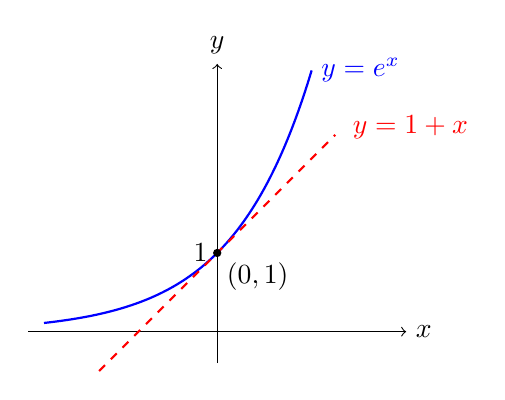
\begin{tikzpicture}[scale=1.0]
\draw[->] (-2.4,0) -- (2.4,0) node[right] {$x$};
\draw[->] (0,-0.4) -- (0,3.4) node[above] {$y$};
\draw[blue, thick, domain=-2.2:1.2, samples=80] plot (\x,{exp(\x)});
\node[blue, right] at (1.2,{exp(1.2)}) {$y = e^{x}$};
% Tangent at x=0: y = 1 + x
\draw[red, thick, dashed, domain=-1.5:1.5, samples=2] plot (\x,{1 + \x});
\node[red, right] at (1.6,2.6) {$y = 1 + x$};
\fill (0,1) circle (1.5pt);
\node[below right] at (0,1) {$(0, 1)$};
\node[left] at (0,1) {$1$};
\end{tikzpicture}
\caption{The exponential \(e^{x}\) and its tangent line at \(x = 0\). The tangent slope at \(0\) is \(e^{0} = 1\), so the tangent line is \(y = 1 + x\) --- the linear approximation \(e^{x} \approx 1 + x\) used throughout calculus and physics for small \(x\).}
\label{fig:exp-tangent-at-zero}
\end{figure}

% expansion:intuition — the slope-equals-value property is the most striking feature of e^x and worth pulling out as a remark; manuscript states it but doesn't dwell on it
\begin{remark}[Self-derivative property]
\Cref{thm:derivative-of-exp} says that \(e^{x}\) coincides with its own derivative function: at every point \(x\), the slope of the graph equals the height of the graph. This is what distinguishes \(e^{x}\) from other exponentials such as \(2^{x}\) or \(10^{x}\): for those, the slope at every point is the height multiplied by a fixed positive constant other than \(1\), so the slope and the height are not equal. The constant \(e\) is precisely the base for which the constant of proportionality is \(1\).
\end{remark}

\begin{remark}[Derivative of \(b^{x}\)]
For a general positive base \(b\), the same calculation gives
\[
\frac{d}{dx}\bigl[b^{x}\bigr] = b^{x} \cdot \ln b,
\]
where the proportionality factor \(\ln b\) (the natural logarithm of \(b\)) reduces to \(1\) exactly when \(b = e\). The derivation routes through the chain rule applied to \(b^{x} = e^{x \ln b}\); we will give it once the chain rule is available.
\end{remark}

% expansion:summary — closing synthesis paragraph linking to §2.5
With the power rule, linearity, and the exponential's self-derivative property, we can now differentiate any polynomial, any constant multiple, any sum, and the exponential function. What we cannot yet differentiate is a product or a quotient of two differentiable functions. The naive guess \((f g)' = f' g'\) fails almost immediately --- the next section produces a small counterexample within its first paragraph --- so the product rule must be derived from scratch from the limit definition. The quotient rule then follows by the same technique with one extra algebraic step.

\section{The Product and Quotient Rules}\label{sec:product-quotient-rules}

% expansion:intuition — section opener pivoting from §2.4's caution that linearity doesn't extend to products
Linearity (\cref{thm:differentiation-linearity}) lets us differentiate sums and constant multiples of differentiable functions term by term. The natural next question is whether the same applies to products and quotients --- whether \((f g)' = f' g'\) and \((f / g)' = f' / g'\). The answer is no, and the very first example shows it.

\subsection{Why \texorpdfstring{$(fg)' \neq f' g'$}{(fg)' is not f'g'}}

Take \(f(x) = x\) and \(g(x) = x^{2}\). Then \(f(x) g(x) = x^{3}\), and by the power rule
\[
(f g)'(x) = (x^{3})' = 3 x^{2}.
\]
On the other hand \(f'(x) = 1\) and \(g'(x) = 2 x\), so
\[
f'(x) g'(x) = 1 \cdot 2 x = 2 x.
\]
The two formulas disagree (compare \(3 x^{2}\) and \(2 x\) at \(x = 1\): \(3\) vs \(2\)). The naive ``differentiate factor by factor'' rule is wrong; the correct formula is the topic of this section.

% expansion:caution — the (fg)' ≠ f'g' pitfall is a recurring source of error throughout the chapter and beyond
\begin{caution}
Differentiation does \emph{not} distribute across multiplication: in general \((f g)' \neq f' g'\), as the example above demonstrates with \(f(x) = x\), \(g(x) = x^{2}\). The correct rule, derived below, is the \emph{product rule} \((f g)' = f' g + f g'\). Students who have absorbed linearity for sums sometimes carry the pattern over to products by analogy; this is the highest-traffic single mistake in introductory differentiation, and the only reliable defence is to remember that the correct formula has \emph{two terms}, not one.
\end{caution}

\subsection{The product rule}

\begin{theorem}[Product rule]\label{thm:product-rule}\index{product rule}
If \(f\) and \(g\) are both differentiable at \(x\), then \(f g\) is differentiable at \(x\), with
\[
(f g)'(x) = f'(x) g(x) + f(x) g'(x).
\]
Equivalently, in Leibniz notation,
\[
\frac{d}{dx}\bigl[f(x) g(x)\bigr] = \frac{df}{dx} g(x) + f(x) \frac{dg}{dx}.
\]
\end{theorem}

\begin{proof}
The difference quotient of \(f g\) at \(x\) is
\[
\frac{f(x + h) g(x + h) - f(x) g(x)}{h}.
\]
The key algebraic step is to add and subtract \(f(x) g(x + h)\) in the numerator, which splits the expression into two pieces each of which has a recognisable difference quotient:
\begin{aligneddisplay}
&f(x + h) g(x + h) - f(x) g(x) \\
&\quad= f(x + h) g(x + h) - f(x) g(x + h) + f(x) g(x + h) - f(x) g(x) \\
&\quad= \bigl(f(x + h) - f(x)\bigr) g(x + h) + f(x) \bigl(g(x + h) - g(x)\bigr).
\end{aligneddisplay}
Dividing by \(h\),
\[
\frac{f(x + h) g(x + h) - f(x) g(x)}{h}
= \frac{f(x + h) - f(x)}{h} \cdot g(x + h) + f(x) \cdot \frac{g(x + h) - g(x)}{h}.
\]
Now take \(h \to 0\). The first factor on the right-hand side tends to \(f'(x)\) by definition. The factor \(g(x + h)\) tends to \(g(x)\) because \(g\) is differentiable at \(x\) and therefore (by \cref{thm:differentiable-implies-continuous}) continuous at \(x\). The factor \(f(x)\) is a constant in \(h\). The factor \((g(x + h) - g(x))/h\) tends to \(g'(x)\). The limit laws for products and sums therefore give
\[
(f g)'(x) = f'(x) g(x) + f(x) g'(x). \qedhere
\]
\end{proof}

% expansion:caution — the use of differentiable-implies-continuous in the proof is an easy step to miss; flag it because students often forget that g(x+h) → g(x) requires g to be continuous
\begin{caution}
The product-rule proof depends on \cref{thm:differentiable-implies-continuous} at the step ``\(g(x + h) \to g(x)\) as \(h \to 0\)''. This step would fail if \(g\) were merely defined at \(x\) without being continuous there, but the hypothesis ``\(g\) differentiable at \(x\)'' implies continuity, so the step is justified. The hidden use of differentiability is a small but load-bearing piece of the proof.
\end{caution}

\begin{workedexample}
\begin{example}\label{ex:product-rule-xex}
Let \(h(x) = x \, e^{x}\). Find \(h'(x)\).
\end{example}

\begin{solution}
With \(f(x) = x\) and \(g(x) = e^{x}\), we have \(f'(x) = 1\) and \(g'(x) = e^{x}\) (\cref{thm:derivative-of-exp}). The product rule gives
\[
h'(x) = f'(x) g(x) + f(x) g'(x) = 1 \cdot e^{x} + x \cdot e^{x} = e^{x} (1 + x). \qedhere
\]
\end{solution}
\end{workedexample}

% expansion:example — supplementary polynomial-product example. Two polynomials multiplied together give an opportunity to compare "expand first, then differentiate" against "product rule directly"; both give the same answer.
\begin{workedexample}
\begin{example}\label{ex:product-rule-poly}
Differentiate \(p(x) = (3 x^{2} + 1)(x^{3} - 4)\) two ways: by expanding before differentiating, and by the product rule.
\end{example}

\begin{solution}
\emph{By expansion.} Expand:
\[
p(x) = 3 x^{5} - 12 x^{2} + x^{3} - 4 = 3 x^{5} + x^{3} - 12 x^{2} - 4.
\]
Differentiate term by term:
\[
p'(x) = 15 x^{4} + 3 x^{2} - 24 x.
\]

\emph{By the product rule.} Set \(f(x) = 3 x^{2} + 1\) and \(g(x) = x^{3} - 4\); then \(f'(x) = 6 x\) and \(g'(x) = 3 x^{2}\). Therefore
\begin{aligneddisplay}
p'(x) &= f'(x) g(x) + f(x) g'(x) \\
      &= 6 x (x^{3} - 4) + (3 x^{2} + 1)(3 x^{2}) \\
      &= 6 x^{4} - 24 x + 9 x^{4} + 3 x^{2} \\
      &= 15 x^{4} + 3 x^{2} - 24 x.
\end{aligneddisplay}
The two methods agree, as they must. The product rule is more efficient when the factors are not polynomials --- expanding \(x e^{x}\), for instance, is not an option. \qedhere
\end{solution}
\end{workedexample}

\subsection{The quotient rule}

The same technique --- a clever add-and-subtract step in the numerator of the difference quotient --- yields the rule for the derivative of a quotient.

\begin{theorem}[Quotient rule]\label{thm:quotient-rule}\index{quotient rule}
If \(f\) and \(g\) are both differentiable at \(x\) and \(g(x) \neq 0\), then \(f / g\) is differentiable at \(x\), with
\[
\left(\frac{f}{g}\right)'(x) = \frac{f'(x) g(x) - f(x) g'(x)}{\bigl[g(x)\bigr]^{2}}.
\]
\end{theorem}

\begin{proof}
The difference quotient of \(f / g\) at \(x\) is
\[
\frac{1}{h}\!\left[\frac{f(x + h)}{g(x + h)} - \frac{f(x)}{g(x)}\right]
= \frac{1}{h} \cdot \frac{f(x + h) g(x) - f(x) g(x + h)}{g(x + h) g(x)}.
\]
Add and subtract \(f(x) g(x)\) in the numerator:
\begin{aligneddisplay}
&f(x + h) g(x) - f(x) g(x + h) \\
&\quad= \bigl(f(x + h) - f(x)\bigr) g(x) - f(x) \bigl(g(x + h) - g(x)\bigr).
\end{aligneddisplay}
Divide by \(h\):
\[
\frac{1}{h}\!\left[\frac{f(x + h)}{g(x + h)} - \frac{f(x)}{g(x)}\right]
= \frac{\frac{f(x + h) - f(x)}{h} g(x) - f(x) \frac{g(x + h) - g(x)}{h}}{g(x + h) g(x)}.
\]
Now take \(h \to 0\). The factor \(g(x + h)\) tends to \(g(x)\) (by continuity), and \(g(x + h) g(x) \to g(x)^{2}\); the differentiated factors tend to \(f'(x)\) and \(g'(x)\). The limit laws give
\[
\left(\frac{f}{g}\right)'(x) = \frac{f'(x) g(x) - f(x) g'(x)}{\bigl[g(x)\bigr]^{2}}. \qedhere
\]
\end{proof}

% expansion:caution — order of f' and g' in the quotient-rule numerator is not symmetric
\begin{caution}
The numerator of the quotient rule is \emph{not} symmetric in \(f\) and \(g\). Swapping the two terms produces a sign error:
\pairdisplay{\text{correct: } f' g - f g',}{\text{wrong:  } f g' - f' g.}
The correct version subtracts \emph{the term containing \(g'\)}; equivalently, the term beginning with \(f'\) comes first. A common memory device is the chant ``low \(d\)-high minus high \(d\)-low, draw the line and square below'' --- in symbols, \(\bigl(\tfrac{\text{high}}{\text{low}}\bigr)' = (\text{low} \cdot \text{high}' - \text{high} \cdot \text{low}') / \text{low}^{2}\). Whatever device works, internalise it: order errors in the quotient rule are the second-most-common differentiation mistake after \((fg)' = f' g'\).
\end{caution}

\begin{workedexample}
\begin{example}\label{ex:quotient-rule-rational}
Differentiate \(\displaystyle q(x) = \frac{x^{2} + 1}{x^{3} - 1}\) wherever the denominator is non-zero.
\end{example}

\begin{solution}
With \(f(x) = x^{2} + 1\) (so \(f'(x) = 2 x\)) and \(g(x) = x^{3} - 1\) (so \(g'(x) = 3 x^{2}\)), the quotient rule gives
\begin{aligneddisplay}
q'(x) &= \frac{f'(x) g(x) - f(x) g'(x)}{g(x)^{2}} \\
      &= \frac{2 x (x^{3} - 1) - (x^{2} + 1)(3 x^{2})}{(x^{3} - 1)^{2}} \\
      &= \frac{2 x^{4} - 2 x - 3 x^{4} - 3 x^{2}}{(x^{3} - 1)^{2}} \\
      &= \frac{-x^{4} - 3 x^{2} - 2 x}{(x^{3} - 1)^{2}}. \qedhere
\end{aligneddisplay}
\end{solution}
\end{workedexample}

% expansion:example — supplementary quotient with the exponential. Pairs naturally with the product-rule example above and shows the rule's reach beyond rational functions.
\begin{workedexample}
\begin{example}
Differentiate \(\displaystyle r(x) = \frac{e^{x}}{x}\) for \(x \neq 0\).
\end{example}

\begin{solution}
With \(f(x) = e^{x}\) (so \(f'(x) = e^{x}\)) and \(g(x) = x\) (so \(g'(x) = 1\)),
\[
r'(x) = \frac{e^{x} \cdot x - e^{x} \cdot 1}{x^{2}} = \frac{e^{x} (x - 1)}{x^{2}}. \qedhere
\]
\end{solution}
\end{workedexample}

% expansion:strategy — rule selection. With a small toolkit of rules in hand, the practical skill becomes deciding which one applies; this is exactly what the "Choosing a differentiation rule" strategy box from the roadmap was for.
\begin{strategy}[Choosing a differentiation rule]
Look at the syntactic shape of the expression to decide which rule applies first:
\begin{enumerate}
    \item \emph{Sum or difference}: differentiate term by term using \cref{thm:differentiation-linearity}.
    \item \emph{Constant multiple}: pull the constant out using \cref{thm:differentiation-linearity}.
    \item \emph{Power}: \cref{thm:power-rule} (positive integer \(n\) for now).
    \item \emph{Product of two non-constant factors}: \cref{thm:product-rule}.
    \item \emph{Quotient of two non-constant expressions}: \cref{thm:quotient-rule}.
    \item \emph{Exponential}: \cref{thm:derivative-of-exp} for \(e^{x}\) (other bases will need the chain rule).
\end{enumerate}
For a complicated expression, the rule applied at the outermost level is the one chosen first; subsequent rules apply to the inner pieces. ``Outermost'' means the operation that would be performed last if the expression were evaluated numerically.
\end{strategy}

% expansion:summary — closing synthesis paragraph for the section, transitioning into the chapter Summary
The product and quotient rules complete the elementary differentiation toolkit: combined with the constant rule, the power rule, linearity, and the derivative of \(e^{x}\), they let us differentiate any expression built from polynomials, the natural exponential, and the four arithmetic operations. What still lies ahead --- the chain rule for compositions, derivatives of trigonometric and inverse-trigonometric functions, derivatives of logarithms, implicit differentiation, and applications such as related rates and optimisation --- builds on top of this foundation, but the foundation itself is now in place.

\section*{Summary}\addcontentsline{toc}{section}{Summary}

% expansion:summary — chapter-end Summary required by CONTENT_SPEC §4. Items are one-line distillations matching the spec's "different depth, different framing" rule.
\paragraph{The derivative as a limit.}
\begin{itemize}
    \item \(\displaystyle f'(a) = \lim_{h \to 0} \frac{f(a + h) - f(a)}{h} = \lim_{x \to a} \frac{f(x) - f(a)}{x - a}\), provided either limit exists.
    \item \(f'(a)\) is the slope of the tangent line at \((a, f(a))\); the tangent line equation is \(y - f(a) = f'(a) \cdot (x - a)\).
    \item Treating the basepoint as a variable yields the derivative function \(f'\); the standard notations \(f'(x), \frac{df}{dx}, \frac{dy}{dx}, \frac{d}{dx}[f(x)]\) all denote the same object.
\end{itemize}

\paragraph{Differentiability and continuity.}
\begin{itemize}
    \item \(f\) is differentiable at \(a\) iff \(f'(a)\) exists; a function may fail to be differentiable at a corner, vertical tangent, or discontinuity.
    \item Differentiable \(\Rightarrow\) continuous (\cref{thm:differentiable-implies-continuous}); the converse is false (\(\lvert x \rvert\) at \(0\)).
    \item Higher derivatives \(f''\), \(f'''\), \(f^{(n)}\) are obtained by iterating differentiation; for a polynomial of degree \(d\), \(f^{(n)} = 0\) for \(n > d\).
\end{itemize}

\paragraph{Differentiation rules.}
\begin{itemize}
    \item Constant: \((c)' = 0\).
    \item Power (positive integer \(n\)): \((x^{n})' = n x^{n - 1}\).
    \item Linearity: \((f + g)' = f' + g'\), \((c f)' = c f'\). (Polynomials differentiate term by term.)
    \item Product: \((f g)' = f' g + f g'\). \emph{Not} \(f' g'\).
    \item Quotient: \(\bigl(\tfrac{f}{g}\bigr)' = \tfrac{f' g - f g'}{g^{2}}\) where \(g \neq 0\). Order in the numerator matters.
    \item Exponential: \((e^{x})' = e^{x}\); the natural exponential is its own derivative.
\end{itemize}

\subsection*{Exercises}

% expansion:summary — exercise inventory deferred per CONTENT_SPEC. Real exercises come from the manuscript; this placeholder respects the Mode A "do not invent exercises" rule.
\emph{Exercises for this chapter are drawn from the manuscript and are deferred to the dedicated exercise pass; see \texttt{CONTENT\_EXERCISES.md}.}

